\newpage
\section{Desarrollo del proyecto}

Para  llevar  a  cabo  el  diseño  y  desarrollo  de  este  proyecto  se  consultaron numerosas  paginas web sobre procesamiento de imágenes y  se  realizaron continuas reuniones con el tutor sobre las dudas que surgían mediante el desarrollo del proyecto.

El principal objetivo de este proyecto es:

\begin{itemize}
\item Hacer uso de un sensor.
\item Recuperar características a través de procesamiento de señales.
\item Utilizar una red neuronal de retropropagación con validación cruzada.
\item Realización de un conjunto de  algoritmos  que  realicen  las  funciones  de  detección  y  reconocimiento  de  patrones de forma eficiente.
\end{itemize}

\subsection{Equipo utilizado}
A continuación se describirá todo  el  material  requerido  para  el  desarrollo  del proyecto, con la finalidad de esclarecer el porqué de la elección de éstos.Se
describirá tanto  el  equipo requerido,  necesario  para  la  instalación  de  programas  y la  simulación de nuestra aplicación, como el software utilizado durante la programación de ésta
\subsubsection{Hardware}
Se han utilizado, dos ordenadores, que cuentan las siguientes especificaciones:
\begin{itemize}
\item Sistema operativo Linux.
\item Procesador Intel Celeron N3060 @ 2x 2.48GHz
\item Memoria Ram de 4GB.
\item 500 GB de memoria de disco duro.
\item Una resolución de pantalla de 1280 x 800.
\end{itemize}

Para la emulación e instalación de nuestra aplicación, también se ha hecho uso de un Smartphone con un sistema operativo Android y cámara incorporada. En este caso se ha utilizado un Smartphone Huawei P10 con la versión de Android 8.

\subsubsection{Software}
\begin{itemize}
\item Android-Studio
\item Libreria OpenCV.
\item Libreria Sclearn
\item Micro framework Flask
\end{itemize}

\subsection{Características de la Aplicación}
El trabajo desarrollado cuenta con las siguientes características:
\begin{itemize}
\item Captura fotografía de un croma y se sube aun servidor.
\item La red neuronal detecta y reconoce si el croma es valido o no.
\item Contiene una interfaz gráfica para facilitar el uso de la aplicación.
\end{itemize}

Todo el procesamiento de imágenes y la red neuronal se ha implementado en python3.


\subsection{Patrones a detectar}

Un croma contiene varias características que determinan si la calidad del suelo se encuentra en buenas condiciones. 

\begin{figure}[H]
 \centering	
   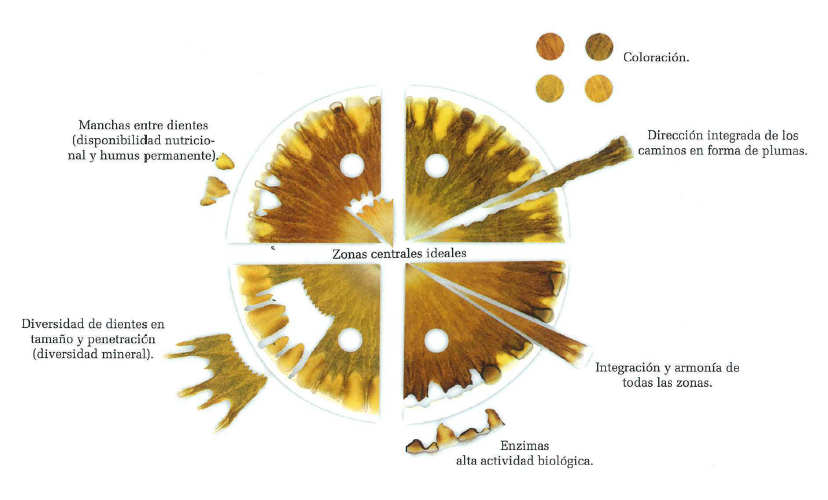
\includegraphics[width=0.8\textwidth]{images/3.png}
   \caption{\textit{Características de un croma.}}
   \end{figure}	
   
Tal y como se observa en la Figura 3, existe una variedad de características que contiene un croma.
El número  de  características a detectar en el programa son ocho que son importantes para saber la calidad del estado del suelo.
Estas características son: 
\begin{itemize}
\item Contorno.
\item Lineas.
\item Colores como el negro, gris, violeta, verde y azul.
\item Dientes de caballo.
\item Patrón de figura (Dientes de caballo)
\end{itemize}

